%
% CHAPTER: Entities, Represenations and Descriptions
%

\chapterimage{owl.pdf} % Chapter heading image

\chapter{Entities, Representations and Descriptions}
\label{cha:Topics-and-Descriptions}

\begin{quote}
\begin{flushright}
\emph{We are all agreed that your theory is crazy. \\
The question which divides us is whether it is crazy enough.} \\
Niels Bohr
\end{flushright}
\end{quote}
\bigskip

The initial step towards quantifying our lack of knowledge involves a precise identification of the research entities under examination. The specific components of this collection depend largely on the specific use case of the nescience theory. Each application necessitates a unique assortment of entities, be it mathematical objects, living organisms, human needs, and so forth. Fortunately, the process of quantifying how much we do not know remains consistent across all cases.

The subsequent step involves devising a methodology to represent the identified entities through strings of symbols, or what we term as 'representations'. Properly symbolizing a research entity is a challenging, yet unresolved, epistemological problem. The solution suggested within the context of nescience theory is rooted in the concept of an oracle Turing machine. The ease of implementing this solution in practice depends largely on the abstract nature of the entities under study. For instance, encoding the entirety of abstract mathematical objects presents significant difficulty, necessitating the discovery of an approximation. In contrast, encoding all possible computer programs (considering our focus on software quality, refer to Chapter \ref{chap:Software-Engineering}) is relatively straightforward, given that computer programs inherently exist as strings.

The final step, once a suitable method of encoding the original entities as string-based representations has been established, requires producing a description. This should be as accurate and concise as possible, detailing our current understanding of these representations. In nescience theory, it's imperative that these descriptions are computable - that is, a computer should be capable of fully recreating the original representation based on the description. A challenge arises with descriptions as they characterize representations, i.e., the encoding of entities, not the entities themselves. Therefore, the effectiveness of a description in representing an entity is contingent upon the quality of the representation used.

In this chapter, we will formalize all these key concepts: entities, representations, descriptions, among others. We will also explore what constitutes a perfect description, how to compute the combined representation of multiple entities, and how to describe a representation assuming another's perfect description. We will further examine the concept of a research area and its properties.

%
% Section: Entities
%

\section{Entities}
\label{sec:descriptions_entities}

Defining the nature of a research entity is an unresolved, intricate philosophical problem. We tackle this complexity from a fundamentally pragmatic perspective. Our theory initiates from the premise that there exists a non-empty collection of \emph{entities}\index{Entities} that we aim to comprehend.

\begin{notation}
We represent the set of research entities of interest as $\mathcal{E}$.
\end{notation}

The exact constituents of $\mathcal{E}$ are contingent on the specific domain in which the theory of nescience is employed, typically aligning with a specific area of knowledge. Instances of entity sets might include: research components in mathematics (abstract); the kingdom of Animalia (living entities); both known and unknown human needs (abstract); all potential computer programs (strings), and so forth. In a strict sense, $\mathcal{E}$ is not a well-defined set, given that it is generally indeterminate what qualifies as a member of this set.

The abstract character of $\mathcal{E}$ affords certain benefits but also imposes significant constraints. The primary constraint is that our definition of nescience is, in most instances, a non-computable quantity, necessitating practical approximations. The chief benefit is that the novel concepts and methods introduced in this book can be applied across a spectrum of problems, not solely restricted to the pursuit of new scientific knowledge.

In the theory of nescience, we preclude the allowance of universal sets, that is, we cannot suppose the existence of a set $\xi$ encompassing everything. The issue with universal sets is that they contravene Cantor's theorem (refer to Example \ref{cantor_theorem}). Cantor's theorem establishes that the power set $\mathcal{P}(\xi)$, constituted by all possible subsets of $\xi$, possesses more elements than the original set $\xi$. This contravenes the assumption that $\xi$ incorporates everything. In nescience theory, the set $\mathcal{E}$ must be indicative of a specific set.

\begin{example}[Cantor's theorem]\index{Cantor's theorem}
\label{cantor_theorem}
Cantor's theorem proposes that for any set $A$, $d(A) < d\left(\mathcal{P}(A)\right)$. Consider $f: A \rightarrow \mathcal{P}(A)$, a function that maps each element $x \in A$ to the set $\{x\} \in \mathcal{P}(A)$; evidently, $f$ is injective, implying $d(A) \leq d\left(\mathcal{P}(A)\right)$. To substantiate that the inequality is strict, let's assume there exists a surjective function $g: A \rightarrow \mathcal{P}(A)$ and consider the set $B = \{ x \in A : x \notin g(x) \}$. As $g$ is surjective, there must exist a $y \in A$ such that $g(y) = B$. This, however, raises a contradiction, $y \in B \Leftrightarrow y \notin g(y) = B$. Consequently, the function $g$ cannot exist, therefore $d(A) < d\left(\mathcal{P}(A)\right)$.
\end{example}

In the theory of nescience, not all conceivable sets are acceptable, as some can lead to paradoxes. Take for example, Russell's paradox, which proposes a set $R$ composed of all sets that are not members of themselves. The paradox emerges when we attempt to discern whether $R$ is a member of itself (refer to Example \ref{ex:russell_paradox}). To circumvent such predicaments, the theory of nescience is founded on the Zermelo-Fraenkel set of axioms\index{Zermelo-Fraenkel set of axioms}, accompanied by the Axiom of Choice\index{Axiom of Choice} (see Appendix \ref{apx:math}). Russell's paradox is attributed to an abuse of the set builder notation $\{ : \}$. The \emph{axiom of separation}\index{Axiom of separation} (if $P$ is a property with parameter $p$, then for any set $x$ and parameter $p$ there exists a set $y=\{u \in x : P(u) \}$ that includes all those sets $u \in x$ having property $P$) permits the use of this notation only to construct sets that are subsets of already existing sets. A broader \emph{axiom of comprehension}\index{Axiom of comprehension} (if $P$ is a property, then there exists a set $y=\{u : P(u) \}$) would be required to permit sets like the one proposed by Russell's paradox. In the ZFC axioms, and within the theory of nescience, the axiom of comprehension is deemed to be false.

\begin{example}[Russell's Paradox]\index{Russell's Paradox}
\label{ex:russell_paradox}
Suppose $R$ is the set of all sets not members of themselves, such that $R = \{ x : x \notin x \}$. The contradiction arises when querying if $R$ is a member of itself. If $R$ is not a member of itself, by its own definition, it should be; conversely, if $R$ is declared to be a member of itself, its definition dictates it should not be. Symbolically, this can be written as $R \in R \Leftrightarrow R \notin R$.
\end{example}

In nescience theory, we do not delve into classical ontological\index{Ontology} queries, i.e., the classification of existent entities in the world that can be known. Additionally, we do not strive to resolve epistemological\index{Epistemology} issues, such as how scientific knowledge is authenticated through evidence or the nature of said evidence.

Once a set $\mathcal{E}$ of entities is chosen, the subsequent step involves uniquely encoding these entities as strings of symbols, otherwise, their description would be impossible (unless the entities themselves are symbol strings). The method to effectively execute this encoding is delineated in the subsequent section.

%
% Section: Representations
%

\section{Representations}
\label{sec:representations}

The conceptualization and depiction of entities within a set $\mathcal{E}$, which may be abstract in nature, pose significant epistemological\index{Epistemology} challenges that have engaged researchers for over two millennia (refer to Section \ref{sec:scientific_representation} for a succinct overview of ongoing issues and unresolved queries). This book outlines a potential resolution to this complex problem, while analyzing its merits and shortcomings. Our proposed approach bifurcates the issue of scientific representation into two interconnected subproblems: the modeling of descriptions into representations, and the encoding of entities into these representations. Thus, scientific descriptions serve to define entities through an indirect association facilitated by representations (refer back to Figure \ref{fig:representationProblem} in the book's introduction, which has been reproduced in this section for convenient referencing). The current section will primarily concentrate on the aspect of encoding, with Section \ref{sec:descriptions_models} focusing on descriptions.

\begin{figure}[t]
\centering
\begin{tikzpicture}
    \node[draw, ellipse, minimum width=3cm] (entities) at (0,0) {Entities};
    \node[draw, ellipse, minimum width=3cm] (representations) at (5,0) {Representations};
    \node[draw, ellipse, minimum width=3cm] (descriptions) at (10,0) {Descriptions};

    \draw[-{Latex[length=3mm]}] (representations) -- node[above,midway] {encode} (entities);
    \draw[-{Latex[length=3mm]}] (descriptions) -- node[above,midway] {model} (representations);
    \draw[dashed,-{Latex[length=3mm]}] (descriptions) to [bend right=45] node[above,midway] {explain?} (entities);
\end{tikzpicture}
\caption{The Problem of Understanding}
\end{figure}

Within the field of Kolmogorov complexity\index{Kolmogorov complexity}, the representation issue is tackled by presupposing that the set $\mathcal{E}$ is well-defined, countable, and that a total encoding function $f:\mathcal{E} \rightarrow \mathbb{N}$ exists, mapping the set of entities to the set of natural numbers (akin to Gödel numbering\index{Gödel numbering}). The nescience theory similarly embraces this concept of encoding entities via numbers, or, in other words, strings of symbols. However, our approach to the problem of encoding an arbitrary set $\mathcal{E}$ involves an inversion of the problem. This involves defining a total function $\mathcal{O}_\mathcal{E}:\mathcal{S}^\ast \rightarrow \mathcal{E}$ that maps the well-defined set $\mathcal{S}^\ast$ (comprising all possible finite strings from an alphabet $\mathcal{S}$) to the potentially non-countable and non-well defined set $\mathcal{E}$ containing the entities of interest.

Our function $\mathcal{O}_\mathcal{E}$, which is contingent upon the set $\mathcal{E}$, operates much like an oracle (taking inspiration from the concept of an oracle Turing machine\index{Oracle Turing machine} as per Definition \ref{def:Oracle-Turing-Machine}). This function has the capacity to entirely reconstruct an entity $\mathcal{O}_\mathcal{E} (x) \in \mathcal{E}$ using its encoding string $x \in \mathcal{S}^\ast$, without the need for additional information. Evidently, this oracle is an abstract concept and its real-world construction would be implausible for most of the sets $\mathcal{E}$. However, the theoretical existence of this oracle assists in the elucidation and verification of key attributes of the scientific discovery process. Due to its oracle-like nature, $\mathcal{O}_\mathcal{E}$ exhibits limitations regarding the mathematical operations it can be employed in, as will be elucidated in the subsequent discourse.

Our premise rests on the assumption of the existence of a singular, distinct physical world that remains uninfluenced by observers. Furthermore, we posit that for certain collections of entities $\mathcal{E}$, it is logically coherent to presuppose the existence of an oracle $\mathcal{O}_\mathcal{E}$ (refer to the discussion on the scientific representation problem in Section \ref{sec:scientific_representation}). For the purposes of this book, without any loss of generality, we will exclusively regard binary strings as the means of encoding entities.

\begin{definition}
\label{def:descriptions_topic}
Given $\mathcal{E}$ as a set of entities, a \emph{representation function}\index{Representation function} is defined as an oracle $\mathcal{O}_\mathcal{E}:\mathcal{B}^\ast \rightarrow \mathcal{E}$ that maps elements of the set $\mathcal{B}^\ast$, which comprises all conceivable finite binary strings, to the elements of the set $\mathcal{E}$, corresponding to the entities under examination.
\end{definition}

Only the elements of the set $\mathcal{B}^\ast$, that is, binary strings, can serve as representations of entities (problem of ontology). We do not allow drawings, or any other form of physical models, unless they are converted into binary strings. We do not make any distinction between a scientific representations and any other kind of representations (demarcation problem). It is up to the oracle to decide which entity is encoded by each representation. It is also important to note that the oracle $\mathcal{O}_\mathcal{E}$ is total, that is, all possible strings represent entities (no targetless models allowed).

Within this framework, only the elements of the set $\mathcal{B}^\ast$, that is, binary strings, are eligible to serve as representations of entities (problem of ontology). We do not permit other forms of physical models, including drawings, unless they can be transcribed into binary strings. We do not distinguish between scientific representations and other forms of representations (demarcation problem). The oracle assumes the responsibility of determining which entity is encoded by each representation. It is also pivotal to note that the oracle $\mathcal{O}_\mathcal{E}$ is total, meaning all potential strings represent entities (models without targets are not permissible).

\begin{example}
\label{ex:not_unique_oracle}
For a given set of entities $\mathcal{E}$, the existence of a representation oracle $\mathcal{O}_\mathcal{E}$ does not imply its uniqueness. For instance, a binary negation oracle (which transforms the zeros of a binary string into ones, and the ones into zeros), assigning to each string $x \in \mathcal{B}^\ast$ the entity $\mathcal{O}_\mathcal{E} \left( \neg x \right)$, would also qualify as a representation function.
\end{example}

Rather than deploying individual oracles, we could have employed a universal oracle machine. This is a machine $\mathcal{U}_\mathcal{O}$ which, given the encoding of an oracle $\mathcal{O}_\mathcal{E}$ and a string $s$ as input, computes $\mathcal{U}_\mathcal{O} \left( \langle \mathcal{O}_\mathcal{E}, s \rangle \right) = \mathcal{O}_\mathcal{E} \left( s \right)$. Universal machines are particularly applicable to the universal set $\xi$, encompassing all entities. However, such an approach would likely complicate the process of scientific discovery in practical terms. We elect instead to work with sets of entities $\mathcal{E}$ corresponding to distinct areas of knowledge, choosing a single oracle $\mathcal{O}_\mathcal{E}$ for each set $\mathcal{E}$ (the most suitable one according to our current understanding).

\begin{example}
\label{ex:description_dna}
Consider the instance when the subjects of study are animals. Initially, we could utilize detailed physical descriptions of the animals as encodings. In this scenario, the oracle would be a hypothetical machine capable of recreating the original animal from its description. As our comprehension of the biology of life advances, we could contemplate the adoption of an alternative encoding based on the animals' DNA. Both these encodings serve as valid representations of the entities.
\end{example}

As illustrated in Example \ref{ex:not_unique_oracle} and Example \ref{ex:description_dna}, the entities of $\mathcal{E}$ could be encoded in various manners (problem of style). Different oracles will accommodate different encoding schemas. Some strings offer superior representations of an entity compared to others (standard of accuracy). The optimal representation is contingent on the type of queries we seek to answer. Employing a specific style of encoding with an oracle that anticipates a different style may yield unforeseen results. Our objective should be to utilize representations that minimize the size of the oracle (i.e., the volume of inherent knowledge presumed to be contained in the oracle).

\begin{example}
Consider $\mathbf{X}_t$ as a time series comprising $m$ measurements $x_1, \ldots, x_m$ gathered at fixed intervals from a physical phenomenon exhibiting sinusoidal behavior, and let's assume we have trained a multi-layer perceptron\index{Multi-layer perceptron} neural network $nn$ that perfectly fits the data, that is, it returns $x_t$ when given a time $t$ as input. An analysis of the time series' cycles will lead us to discern that the most appropriate model for this particular physical phenomenon appears to be a sine function. Nonetheless, no extant machine learning methodology would reach the same conclusion when provided with the architecture of the neural network (number of layers, sizes, and trained weights) as input. Clearly, the oracle is so sophisticated that it can, indeed, achieve this.
\end{example}

Remember that the oracle functions as a total function, implying that every conceivable string must represent an entity, even the incomplete ones. The more information a representation lacks, the more challenging it becomes for us to decipher the functioning of the oracle. It's crucial to exercise caution with representations that don't capture the entirety of the original entities, as the results of our analyses could exhibit bias. Chapter \ref{chap:Miscoding} provides an in-depth exploration of errors attributed to the miscoding of abstract entities, illustrating that not only must representations pertain to entities, but also that entities must be relevant to representations (requirement of directionality).

We employ an oracle function as opposed to an oracle relation $\mathcal{R}_\mathcal{O} \subset \mathcal{B}^\ast \times \mathcal{E}$, not with the aim of pairing strings with their corresponding entities, but to construct an entity given its representation. The oracle's capacity to reconstruct original entities legitimizes our ability to formulate hypotheses about entities based on their representations (surrogative reasoning). According to the theory of nescience, scientific investigation involves not only discerning how to encode entities appropriately, but also uncovering the intricacies of the decoding oracles. 

The purpose of encoding entities in the theory of nescience differs from that of Shannon's information theory, as illustrated in Example \ref{ex:shannon_encoding}.

\begin{example}
\label{ex:shannon_encoding}
Take, for instance, a set $\mathcal{E}$ comprising two books: "The Ingenious Nobleman Sir Quixote of La Mancha" and "The Tragedy of Romeo and Juliet". We could encode the first book with the string "0" and the second with the string "1". While these strings allow us to uniquely identify each book in the set, they don't qualify as suitable encodings in the context of the theory of nescience. Information theory is about identifying an object uniquely given a reference, necessitating mutual agreement between the sender and receiver about the mapping between references and objects. On the other hand, in the theory of nescience, we're interested in providing a representation that encapsulates all the nuances and details of the original objects. For instance, it's impossible to hypothesize about Cervantes' influence on Shakespeare's work given the strings "0" and "1".
\end{example}

An alternative approach to addressing the problem outlined in Example \ref{ex:shannon_encoding}, where we used artificially brief descriptions, could involve demanding the set $\mathcal{E}$ to be infinite, as Kolmogorov complexity does (thereby precluding infinite instances of deception). However, even with an infinite set of entities, not every possible encoding schema can ensure the satisfaction of the highly desirable property of surrogative reasoning.









We distinguish between \emph{knowable} and \emph{unknowable} entities.

\begin{definition}
We say that an entity $e \in \mathcal{E}$ is \emph{knowable} if there exists at least one $r \in \mathcal{B}^\ast$ such that $\mathcal{O}_\mathcal{E}(r) = e$. An entity $e \in \mathcal{E}$ is \emph{unknowable} if it is not knowable.
\end{definition}

A priori, it is not possible to determine if a set of entities $\mathcal{E}$ is knowable, unknowable, or partially knowable. Selecting the right knowable entities to study is a matter of trial and error. In this book we have nothing to say about unknowable entities, beyond that the unknowability of an entity cannot be proved nor discovered.

\begin{definition}
Let $e \in \mathcal{E}$ a knowable entity. We call the \emph{set of representations} for $e$, denoted by $\mathcal{R}_e$, to $\{ r \in \mathcal{B}^\ast : \mathcal{O}_\mathcal{E} (e) = r \}$.
\end{definition}

In figure \ref{fig:entities_topics_1} we have a representation of an hypothetical oracle from the set of finite binary strings $\mathcal{B}^\ast$ to the set of entities $E$; we have also depicted a particular entity $e_1$, the subset of strings $\mathcal{R}_{e_1}$ that encode that entity, and a particular representation $r_1$. Since the set $\mathcal{E}$ is, in general, not well defined, the inverse function $\mathcal{O}_\mathcal{E}^{-1}(e_1)$ cannot be computed in practice.

\begin{figure}[h]
\centering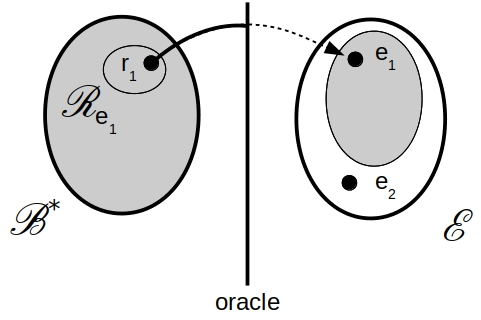
\includegraphics[scale=0.5]{entities_topics_1}
\caption{\label{fig:entities_topics_1}Encodings and Entities.}
\end{figure}

A consequence of working with finite strings as representations is that it might happen that there exist entities that are not encoded by any representation (see the gray areas in Figure \ref{fig:entities_topics_1}, in particular, the entity $e_2$ is not encoded by any representation). Intuitively, we could say that for some domains of knowledge the number of problems is much higher than the number of solutions.

\begin{example}
If the collection of entities under study are real numbers, it turns out that there exist numbers that can not be encoded using finite binary strings, since the set $\mathbb{R}$ has the cardinality of the continuum, and the set $\mathcal{B}^\ast$ is numerable.
\end{example}

Since our knowledge about the entities and the inner workings of the oracle are incomplete, in practice we will working with another set of strings that we believe are close to the representations $\mathcal{R}_e$ that encode the entity $e$. The elements that belong to this set usually change over time, as we better understand the entities of $\mathcal{E}$, and how the oracle encode these entities as strings. The more abstract is our set of entities, the more difficult will be to approximate them as strings (see Chapter \ref{chap:Miscoding}).

\begin{example}
\label{ex:luminiferous_ether}
The entity "luminiferous ether" was a theoretical postulate about a hypothetical medium in which the light would propagate. The ether was used as an explanation of how a wave-based light could propagate through the empty space. In 1887, the results of the Michelson-Morley experiment suggested that the ether did not exist, and after Einstein formulated his special theory of relativity, that successfully explained how light propagates through empty space, the idea of ether was completely dropped.
\end{example}

If the selected oracle is not minimal, finding what it is exactly a valid representation will require to understand how the oracle works internally. By non-minimal oracle we mean that part of the information required to reconstruct the original entity is hard-wired in the oracle itself, instead of encoded as symbols in the representations. Working with non-minimal oracles could make the research process easier.

\begin{remark}
One of the problems of science, and in general of any human intellectual activity, is that people tend to confuse symbols with what they represent. The theory of nescience has been carefully designed to avoid this problem, by means of clearly stating the difference between research entities and the representation of entities. However, keeping this distinction always explicit in the explanations would make the book very difficult to read. We have tried to find a compromise between clarity in the exposition and rigor in the definitions. Sometimes, during the introduction of new ideas we talk in general about a \emph{topics}, meaning an entity, a representation, or both, an entity and its representation. But, in the mathematical definitions and propositions we always make this difference unequivocal. In case of doubt about what we mean, please take the mathematical definitions as the authoritative reference. 
\end{remark}

%
% Section: Invalid Representations
%
\section{Invalid Representations}
\label{sec:invalid_representations}

It might happen that the representation we are using for an entity $e \in \mathcal{E}$ is an incorrect one, that is, instead of working with a string $r \in \mathcal{B}^\ast$ that perfectly encodes $e$, we are studying another string $r' \in \mathcal{B}^\ast$ that it is, hopefully, close to $r$ but not necessarily equal. We are interested in to compute the distance between the string $r'$ and the perfect one $r$ as a quantitative measure of the error we are introducing due to the use of a wrong encoding. Unfortunately, we do not know $r$, since for the majority of the practical applications, it does not exists a computable function from $\mathcal{E}$ to $\mathcal{B}^\ast$. The only thing we have to our disposal is an abstract oracle machine $\mathcal{O}_\mathcal{E}$ that knows which strings represents each entity. Recall from Section \ref{sec:representations} that we propose to address the scientific representation problem by introducing an abstract oracle $\mathcal{O}_\mathcal{E}:\mathcal{B}^\ast \rightarrow \mathcal{E}$ from the set $\mathcal{B}^\ast$ of all possible finite binary strings to the set $\mathcal{E}$ of entities under study.

We start by distinguishing between valid representations, that is strings that contain all the relevant information required by the selected oracle to reconstruct an entity, and non-valid representations.

\begin{definition}
Let $\mathcal{E}$ be a collection of entities, and $\mathcal{O}_\mathcal{E}$ an encoding function. We define the set of \emph{valid} representations for $\mathcal{E}$ given the encoding function $\mathcal{O}_\mathcal{E}$, denoted by $\mathcal{R}^\star_{\mathcal{O}_\mathcal{E}}$, as the subset of representations that perfectly encode an entity of $\mathcal{E}$, according to $\mathcal{O}_\mathcal{E}$.
\end{definition}

The set $\mathcal{R}^\star_{\mathcal{O}_\mathcal{E}}$ is, in general, unknown, since it is a subset of $\mathcal{B}^\ast$ whose definition depends on an abstract, not well defined, oracle. Intuitively, a representation is valid if it contains all the details required so that the oracle can reconstruct the original entity without requiring the use of external information. A valid representation cannot contain wrong symbols nor relevant information can be missing, since in that case the oracle would not be able to reconstruct the entity. Moreover, we require that the oracle is not only able to reconstruct an entity given a representation but it can also derive the set of valid representations given an entity. In this sense, an entity that contains non-relevant information cannot be valid, since that part of the string cannot be generated by the oracle given the entity.

\begin{example}
The data used in time of Ptolomeo about the position of celestial bodies along the year was a non-valid encoding of the entity "position of celestial bodies", since the data was inaccurate. A better encoding was the data collected by Tycho Brahe. Today, we have even better encodings. Adding to the dataset the name of the person who collected the data is an example of a representation that includes non-relevant information.
\end{example}

Recall that we do not allow other representations of entities except finite binary strings. Drawings, mathematical formulas, or datasets can be used as representations as long as they can be encoded as strings and are recognized as valid representations by the selected oracle. Each string represents one, and only one entity. Of course, different oracles will define different sets of valid representations. In general, we will assume that a particular representation oracle $\mathcal{O}_\mathcal{E}$ has been selected to encode the set $\mathcal{E}$ of entities in which we are interested.

\begin{notation}
We will denote the set of valid representations of $\mathcal{E}$ by $\mathcal{R}^\star_\mathcal{E}$ if there is no ambiguity about which oracle $\mathcal{O}_\mathcal{E}$ we are using.
\end{notation}

We can define the set of valid representations of a single entity $e$ in the same way.

\begin{definition}
We define the set of valid representations for an entity $e \in \mathcal{E}$, denoted by $\mathcal{R}^\star_e$, as the subset of representations that perfectly encode the entity $e$, that is, $\mathcal{R}^\star_e = \mathcal{R}^\star_\mathcal{E} \cap \mathcal{R}_e$.
\end{definition}

As we have seen in Example \ref{ex:description_dna} there could be more than one valid representation for some entities, even it the oracle is restricted to a particular style. It might also happen that the set of valid representations is empty, that is, there is no valid representation for that entity. In that case the entity will be unknowable.

\begin{notation}
We denoted by $r^\star_e \in \mathcal{R}^\star_\mathcal{E}$ the fact that $r$ is a valid representation of the entity $e$.
\end{notation}

All possible strings represent an entity, even the non-valid representations, like wrong or incomplete ones. A consequence of working with approximations instead of the true representations is that some of the candidate strings currently in use might encode a different entity from what we were expecting.

\begin{example}
\label{ex:polywater}
In 1961, the Soviet physicist Nikolai Fedyakin, performed a series of experiments resulting in what was seemingly a new form of water. The new water, called polywater, showed a higher boiling point, a lower freezing point, and much higher viscosity than ordinary water. Later experiment showed that polywater was nothing more than contaminated water with small amounts of impurities.
\end{example}

{\color{red}

We can safely assume (it is free from logical contradictions) that the oracle machine not only knows which representations encode which entities, but also how far is a string $r$ from being a valid representation $r^\star_e$, for all $r \in \mathcal{B}^\ast$ and all $r^\star_e \in \mathcal{R}^\star_\mathcal{E}$. 

If a representaton $r$ is non-valid, the oracle will find the closest possible representation that it is valid, and assume that they represent the same entity.

The oracle defines an equivalence relation that splits the set $\mathcal{L}$ into equivalence classes. Each equivalence class corresponds to an entity of $\mathcal{E}$, and it might happens that not all entities of $\mathcal{E}$ have an associated class (what we have called the unknowable unknown). All the strings are related to some entity, and some of them would be better than others (i.e. lower nescience). No string can be part of two different entities. For each collection of $\mathcal{E}$ there could be more than one valid oracle.

\begin{proposition}
Axioms A1, A2 and A3 state that the oracle $\mathcal{O}$ is an equivalence relation
\begin{itemize}
\item[A1] $\forall t \in \mathcal{L} \; t \mathcal{O} t$.
\item[A2] $\forall s , t \in \mathcal{L}$ if $s \mathcal{O} t$ then $t \mathcal{O} s$.
\item[A3] $\forall r, s , t \in \mathcal{L}$ if $r \mathcal{O} s$ and $s \mathcal{O} t$ then $r \mathcal{O} t$.
\end{itemize}
\end{proposition}

\begin{definition}
Let $\mathcal{L} / \mathcal{O}$ be the quotation set defined by the oracle relation over the language set. We call \emph{entity}, denoted by $[e]$, to every class of this quotation set, that is, $[e] \in \mathcal{L} / \mathcal{O}$.
\end{definition}

}

%
% Section: Joint Representations
%

\section{Joint Representations}
\label{sec:descriptions_joint_topic}

We have seen in the previous section that there exists more than one way to encode an entity $e \in \mathcal{E}$, what we have called the set $\mathcal{R}_e$ of representations of the entity. Some of these representations have a high quality, in the sense that they contain all the information required by the oracle to reconstruct (in whatever way the oracle manages to do that) the original entity. But also, in the set $\mathcal{R}_e$ there exists low quality representations, that is, representations that lack many of the details needed to fully reconstruct the entity. Furthermore, the set $\mathcal{R}_e$ can contain representations that include information that is wrong, symbols that the oracle will automatically ignore during the reconstruction, but that they will mislead us when understanding the entity. In Chapter \ref{chap:Miscoding} we will study how to measure the error due to incomplete and wrong representations, and in this section we will introduce a mechanism to improve our currently known representations.

If we want to increase our knowledge about an entity, we have to find the best possible representation for that entity, that is, a representation that is complete and correct. One way to do that is simply try different strings until we come up with a high quality representation. However, that method could require a lot of time and it is impractical. A more efficient approach would be to complement our current bad representation with more (potentially missing) symbols, or by combining those known representations that contain partial information. These two methods require the introduction of the concept of joint representation.

\begin{definition}
Let $s, t \in \mathcal{B}^\ast$ be two different representations. We call \emph{joint representation} of $s$ and $t$ to the concatenation string $st$.
\end{definition}

\begin{example}
\label{ex:lung_cancer}
{\color{red} TODO: use an example in which we talk about concatenating two representations, but do not mention the quality of the individual and joint representations (this is covered in the chapter of miscoding)}
Suppose that the research entity $e$ in which we are interested is the causes of lung cancer. In order to understand this entity, we have measured a collection of risk factors in a random sample of the population (smooking, exercise, diet, age, etc.). However, due to a problem with the sampling procedure, all the samples correspond to a subset of the population, for example, males. This dataset would be a representation $s$ for our entity $e$, but a very bad one, since it is strongly biased. If we have a second representation, corresponding the sample data of females $t$, the joint representation $st$ will be a better one that any of them, $s$ or $t$, isolated.
\end{example}

The concatenation of any two arbitrary representations is also a representation.

\begin{proposition}
Let $s, t \in \mathcal{B}^\ast$ be two different representations and $st$ its joint representation, then $st$ is also a representation.
\end{proposition}
\begin{proof}
As we have seen in Section \ref{sec:strings} the set $\mathcal{B}^\ast$ is closed under the operation of concatenation of strings, and the representation function $\mathcal{O}_\mathcal{E}$ is total.
\end{proof}

We do not require the set of representations $\mathcal{R}_e$ for a given entity $e \in \mathcal{E}$ to be closed under the operation of concatenation. That is, it might happen that $st \notin \mathcal{R}_e$, even if it is the case that $s \in \mathcal{R}_e$ and $t \in \mathcal{R}_e$.

The concept of joint representation is defined for every pair of strings $s, t \in \mathcal{B}^\ast$, even if they do not belong to the same set of representations $\mathcal{R}_e$, in other words, when $\mathcal{O}_\mathcal{E} \left( s \right) \neq \mathcal{O}_\mathcal{E} \left( t \right)$. This process of joining representations from different entities will be very usefull for the discovery of new research entities hitherto unknown (see Section \ref{sec:New_Research_Topics} and recall that all possible strings in $\mathcal{B}^\ast$ represent an entity).

The operation of string concatenation is associative, that is, $(rs)t = r(st)$, for all $r, s, t \in \mathcal{B}^\ast$. This property defines the algebraic structure of the sets of representations.

\begin{proposition}
The set $\mathcal{B}^\ast$ of representations together with the operation of concatenation has the structure of free monoid.
\end{proposition}
\begin{proof}
As we have seen in Section \ref{sec:strings} the operation of string concatenation in $\mathcal{B}^\ast$ is associative, and the empty string $\lambda$ plays the role of neutral element.
\end{proof}

We do no require the operation of joining representations to be conmutative with respect to the oracle function. Given the representations $s, t \in \mathcal{B}^\ast$ it might happen that the concatenation strings $st$ and $ts$ represent different entities, that is, $\mathcal{O}_\mathcal{E} \left( st \right) \neq \mathcal{O}_\mathcal{E} \left( ts \right)$.

The concept of joint representation can be extended to any arbitrary, but finite, collection of representations. In this way, we could add multiple partial representations to our research, or use them in the process of discovering new entities.

\begin{definition}
Let $r_1, r_2, \ldots, r_n \in \mathcal{B}^\ast$ be a finite collection of representations. We call \emph{joint representation} of $r_1, r_2, \ldots, r_n$ to the string $r_1 r_2 \ldots r_n$.
\end{definition}

It is easy to show that $r_1 r_2 \ldots r_n \in \mathcal{B}^\ast$ for all $r_1, r_2, \ldots, r_n \in \mathcal{B}^\ast$, that is, $\mathcal{B}^\ast$ is closed under the operation of concatenation of multiple, finite, representations.

{\color{red}

We have seen that the contatenation of two or more representations of an entity can encode a different entity than the original one. This can even happen when the two representations to join encode the same entity.

multiple representations of the same entity can help us to find a better representation. We can take advantage of this property to discover new, previously unknown entities, by means of combining the representations of the already known entities. Intuitively, we are looking for new entities by creating new representations that are different from the representations we already know.

TODO: Formalize this idea with a proposition.

Provide an example of how it can be applied in practice.

}

%
% Section: Descriptions
%

\section{Descriptions}
\label{sec:descriptions_models}

So far, our aim with the strings of $\mathcal{B}^\ast$ has been to provide an enconding, or representation, as complete and detailed as possible of the entities of $\mathcal{E}$, no matter its length. However, as we have said in the preface of this book, human understanding requires the derivation of concise models for those entities, since human reasoning cannot be based on long representations.

\begin{example}
In Example \ref{ex:lung_cancer} we have shown that a good representation for the entity "lung cancer" could be a sample dataset in which we measure different risk factors. If smokers decide to quit smooking is not because they know and understand this large sample dataset, but because they know and understand the much simpler derived model "smooking increases the risk of lung cancer".
\end{example}

A description or model\footnote{In the theory of nescience use the words "description" and "model" interchangeably.} is a finite binary string mapped to a representation of an entity (recall Figure \ref{fig:entities_topics_models} from Chapter \ref{chap:Introduction}). Descriptions do not model entities (target systems) directly, they do so through string based representations. In the theory of nescience we require that descriptions must be computable, so we can fully and effectively reconstruct the original representations given their descriptions. The requirement of computability allows us to clearly state the limits of the concept of "description". For example, the problem of self-referential descriptions, like the Berry paradox\index{Berry paradox}, can be addressed in the scope of the limits of computation.

\begin{definition} [Model]
\label{def:descriptions_model}
Let $d \in \mathcal{B}^\ast$ be a binary string in the form $d = \langle TM,a \rangle$, where $TM$ is the encoding of a prefix free Turing machine and $a$ is the input string to that machine. If $TM(a)$ is defined, we say that $d$ is a \emph{description}\index{Description}. 
\end{definition}

Intuitively, a description is composed by two parts, a Turing machine that should compresses all the regularities found in this representation, and a string containing what is left, that is, the non-compressible part.

\begin{definition}
\label{def:descriptions_model}
We define the \emph{set of descriptions}\index{Set of descriptions}, denoted by $\mathcal{D}$, as:
\[
\mathcal{D} = \{ d \in \mathcal{B}^\ast : d = \langle TM,a \rangle \wedge TM(a) \downarrow \}.
\]
Let $r \in \mathcal{B}^\ast$ be a representation. We define the set of \emph{descriptions for $r$}, denoted by $\mathcal{D}_r$, as:
\[
\mathcal{D}_r = \{ d \in \mathcal{D} : TM(a) = r \}.
\]
Finally, given an entity $e \in \mathcal{E}$, we define the set of \emph{descriptions for $e$}, denoted by $\mathcal{D}_e$, as:
\[
\mathcal{D}_e = \{ d \in \mathcal{D} : \exists r \in \mathcal{R}_e,\, TM(a) = r \}.
\]
\end{definition}

From an otological point of view, descriptions are just string based representations that satisfy the additional requirement of being computable. In this sense, descriptions are also representations, and so, there exists descriptions that describe descriptions. In practice it is not a good idea to use descriptions as the representation of entities, since what we are looking for in a good representation is that they contain as many details as possible about the original entities, not a concise encoding. Working with descriptions in the role of representations would make the job of scientific discovery very difficult for humans.

Since each description describes one, and only one, representation, we can define a function that maps descriptions into representations. Given that descriptions are Turing machines, it is natural to use as description function a universal Turing machine. Consequently, not only the individual descriptions of representations are computable, but also the function that maps descriptions into representations is also computable.

\begin{definition}
We call \emph{description function}\index{Description function}, denoted by $\delta$, to any universal Turing machine $\delta : \mathcal{D} \rightarrow \mathcal{B}^\ast$ that maps descriptions to their corresponding representations.
\end{definition}

If $d = \langle TM, a \rangle$ is a description of the representation $r$, then we have that $\delta \left( d \right) = \delta \left( \langle TM, a \rangle \right) = TM(a) = r$.

Inspired by the Occam's razor principle\index{Occam's razor principle}\footnote{The Occam's razor principle refers to the number of assumptions of an explanation, not to the length of the explanation itself.}, if two explanations are indifferent, we should prefer the shortest one. Therefore, the limit of what can be known (understand) about a representation, that is, its perfect model, is given by the shortest description that allows us to reconstruct this representation.

\begin{definition}
\label{def:descriptions_perfect_model}
Let $\mathcal{D}_r$ be the set of descriptions of a representaton $r \in \mathcal{B}^\ast$, and let $d \in \mathcal{D}_r$ be a description of $r$. We say that $d$ is a \emph{perfect description}\index{Perfect description} of the representation $r$ if there is no other description $d' \in\mathcal{D}_r$ such that $l(d') < l(d)$.
\end{definition}

Recall that what we know about an entity $e$ is conditional to the quality of the representation $r$ used. If the representation $r$ is wrong, we cannot reach a perfect knowledge about $e$ even if we have found the perfect description $d$ for $r$.

\begin{notation}
We donote by $d_r^{\star}$ the fact that the description $d$ is a perfect description for the representation $r$.
\end{notation}

The perfect description for a representation might not be unique, that is, there could be more than one optimal way to compute $r$.

\begin{definition}
\label{def:set_descriptions_perfect_model}
Let $\mathcal{D}_r$ be the set of descriptions of a representaton $r \in \mathcal{B}^\ast$. We define the \emph{set of perfect descriptions} for $r$, denoted by $\mathcal{D}^\star_r$, as the subset of $\mathcal{D}_r$ composed by the perfect descriptions of $r$.
\end{definition}

Unfortunately, the set of perfect descriptions of a representation is in general not known and, as Proposition \ref{prop:nescience-kolmogorov} shows, there exist no algorithm to compute it. In practice what we have to do is to use an approximation to estimate how far our current best description is from a perfect one, that is, how much we do not know about a particular representation for an entity (see Chapter \ref{chap:Redundancy}).

\begin{proposition}
\label{prop:nescience-kolmogorov}
Let $r \in \mathcal{B}^\ast$ be a representation and $d_r^{\star}$ be a perfect description, then we have that $l \left( d_r^{\star} \right) = K\left( r \right)$.
\end{proposition}
\begin{proof}
Apply Definition \ref{def:Kolmogorov-Complexity} and the fact that we require that the Turing machines $TM$ used in definitions $\langle TM,a\rangle$ must be prefix-free.
\end{proof}

The actual length of a description $l \left( d \right)$ for a representation $r$ is something that depends on the particular enconding of Turing machines used. The encoding method is given by the description function $\delta$ used. Fortunately, if we replace our description function by a different one, the length of perfect models do not change (up to an additive constant that does not depend on the representations themselves).

\begin{corollary}
Let $r \in \mathcal{B}^\ast$ be a representation, $\delta$ and $\dot{\delta}$ two different description functions, and $d_r^{\star}$ the perfect description of the representation $r$ using $\delta$ and $\dot{d}_r^{\star}$ the perfect description using $\dot{\delta}$, then we have that $l \left( d_r^{\star} \right) \leq l \left( \dot{d}_r^{\star} \right) + c$ where $c$ is a constant that does not depend on $r$.
\end{corollary}
\begin{proof}
Apply Theorem \ref{prop:nescience-kolmogorov} and Theorem \ref{def:Invariance-theorem}.
\end{proof}

In general, in the theory of nescience we are not interested in computing the actual value of the nescience about an entity given a description and a representation. Instead what we are interested is in the ordering of the different possible pairs of descriptions and representations given their nescience. In this sense, the details of the particular universal Turing machine used in practice are not relevant\footnote{Do not confuse the inner workings of the universal Turing machine that maps descriptions to representations, in which we are not interested, with the inner workings of the universal oracle Turing machine that maps representations to entities, in which we are interested, since this knowledge is critical to understand how things work.}. For the rest of this book we will assume that $\delta$ is fixed to a reference universal Turing machine. For example, in Section \ref{sub:ax_type_theory} we use as univeral Turing machine the lambda calculus. Alternatively, the reader could consider that all the theorems provided in this book that deal with the length of shortest models are valid up to an additive constant that does not depend on the topics themselves.

A remarkable consequence of Proposition \ref{prop:nescience-kolmogorov} is that perfect descriptions must be incompressible, that is, \emph{perfect knowledge implies randomness} (see Section \ref{sec:incompressibility_randomness}).

\begin{corollary}
Let $d_r^{\star}$ be the perfect description of a representation $r$, then we have that $K \left( d_r^{\star} \right) = l \left( d_r^{\star} \right)$.
\end{corollary}
\begin{proof}
Having $K \left( d_r^{\star} \right) < l \left( d_r^{\star} \right)$ would be a contradiction with the fact that $d_r^{\star}$ is the shortest possible description of $r$.
\end{proof}

The converse, in general, does not hold, since we could have a random description that it is not the shortest possible one, that is, a description $d$ for a reprsentation $r$ such that $l(d) = K(d)$ but $l(d_r^{\star}) < l(d)$.

\begin{example}
\label{ex:description_neural}
We could define a deep neural network\index{Neural network} with an input layer of one thousands nodes, ten hidden layers of fifty thousands nodes each, and an output layer of one thousand nodes, and then train the network to output a fixed string of one thousand 1's for any given input string. The Kolmogorov complexity of this neural network is much higher that the complexity of a string of one thousand 1's.
\end{example}

There is little value on descriptions that are longer than the representations they describe, that is, descriptions that do not compress the representations.

\begin{definition}
\label{def:trivial_model}
Let $r \in \mathcal{B}^\ast$ be a representation, and $d \in \mathcal{D}_r$ one of its descriptions. If $l(d) \geq l(r)$, we say that $d$ is a \emph{pleonastic description}\index{Pleonastic description} of the representation $r$.
\end{definition}

\begin{example}
\label{ex:topics_models_graph}
Consider the set of all possible finite graphs\index{Graph}. Since graphs are abstract mathematical objects, we need a way to represent them as strings, for example, by using a binary encoding of their adjacency matrices (see Section \ref{sec:Graphs} for an introduction to graphs). The description $d = \langle TM, r \rangle$, where $r$ is the representation of a graph and $TM$ is a Turing machine that just halts, will be part of $\mathcal{D}_r$ since $TM(r) = r$. We are concerned about the fact that this description may not be shortest possible description of $r$.
\end{example}

It might happen that there is no shortest possible description of a representation than the representation itself. This is the case when representations are random, or incompressible, strings. And, as we have seen in Section \ref{sec:incompressibility_randomness} the overhelming majority of strings are incompressible. It is useless to do research about random representation, since it is not possible to find shorter models for that representation.

The concept of perfect description can be generalized from individual representations to entities. This generalization allow us to study the nature and properties of these entities.

\begin{definition}
\label{def:entities_perfect_model}
Let $\mathcal{D}_e$ be the set of descriptions of an entity $e \in \mathcal{E}$. We define the \emph{set of perfect descriptions} of the entity $e$, denoted by $\mathcal{D}^\star_e$ as the subset of $\mathcal{D}_e$ composed by perfect descriptions. The elements of $\mathcal{D}^\star_e$ are denoted by $d^\star_e$.
\end{definition}

If $d^\star_e \in \mathcal{D}^\star_e$ there must exits a $r \in \mathcal{R}^\star_e$ such that $d^\star_e \in \mathcal{D}^\star_r$.

An interesting case is when all the descriptions that compose $\mathcal{D}_e$ are pleonastics, that is, there is no model that it is shorter than the representation for all the possible representations of the entity. That would the case if all the representations of the entity $e$ are random strings. In this particular case, scientific research would be doomed, since it is not possible to find a suitable model for $e$. The fact that we can understand and make predictions about $e$ will be limited by the length of the non-compressible representations of $e$.


%
% Section: Models for Joint Representations
%

\section{Descriptions for Joint Representations}
\label{sec:description_joint_represenation}

In Section \ref{sec:descriptions_joint_topic} we introduced the concept of joint representation $ts$ of two individual representations $t$ and $s$. In this section we are interested in to study how the length of the perfect description of a joint representation relates to the length of the perfect descriptions of the individual representations.

The length of the perfect description of a joint representation is greater or equal than the length of the perfect description of the individual representations. That is, the more information we include in a representation, the longer will take to describe it. 

\begin{proposition}
\label{prop:joint_length}
Let $t,s \in \mathcal{B}^\ast$ be two representations and $m_{t}^{\star}$, $m_{s}^{\star}$ and $m_{ts}^{\star}$ the perfect descriptions of the representatons $t$, $s$ and the joint representation $ts$ respectively. We have that $l \left( m_{ts}^{\star} \right) \geq l \left( m_{t}^{\star} \right)$ and $l \left( m_{ts}^{\star} \right) \geq l \left( m_{s}^{\star} \right)$.
\end{proposition}
\begin{proof}
The statement $l \left( m_{ts}^{\star} \right) \geq l \left( m_{t}^{\star} \right)$ is equivalent to $K(ts) \geq K(t)$. Then apply Proposition \ref{prop:excess_kolmogorov}.
\end{proof}

Intuitively, adding more information to a representation is a good thing if this information is relevant to describe the entity in which we are interested. But adding non-relevant information will make our model unnecessarily long. Recall that the process of joining representations can be used to concatenate two partial representations of the same entity, or to extend a representation with additional missing symbols.

If the selected representations partially overlap, we could take advantage of this redundancy to come up with a shorter join description than simply joining the individual descriptions. In the worst case, the perfect description of a joint representation would be the concatenation of the perfect descriptions of the individual representations.

\begin{proposition}
\label{prop:joint_sum}
Let $t,s \in \mathcal{B}^\ast$ be two representations and $m_{t}^{\star}$, $m_{s}^{\star}$ and $m_{ts}^{\star}$ the perfect descriptions of the representatons $t$, $s$ and the joint representation $ts$ respectively. We have that $l \left( m_{ts}^{\star} \right) \leq l \left( m_{t}^{\star} \right) + l \left( m_{s}^{\star} \right)$.
\end{proposition}
\begin{proof}
The statement $l \left( m_{ts}^{\star} \right) \leq l \left( m_{t}^{\star} \right) + l \left( m_{s}^{\star} \right)$ is equivalent to $K(ts) \leq K(t) + K(s)$, then apply Proposition \ref{prop:additive_kolmogorov}.
\end{proof}

{\color{red} An interpretation of Proposition \ref{prop:joint_sum} is that including redundant information in the representation of an entity is not a problem from the point of view of finding its shortest possible description. In practice, we have to use that representation that makes the process of scientific discovery (finding the best model) as easy as possible, even if this representation is unnecessarily long. In contrast, Proposition \ref{prop:joint_length} claims that adding non-relevant symbols to a representation is something that has to be avoided.}

Finally, next proposition proves that the order of the representations in the perfect description of a joint representation does not change its length.

\begin{proposition}
\label{prop:joint_order}
Let $t,s \in \mathcal{B}^\ast$ be two representations and $m_{ts}^{\star}$ and $m_{st}^{\star}$ the perfect descriptions of the joint representations $ts$ and $st$ respectively. We have that that $l \left( m_{ts}^{\star} \right) = l \left( m_{st}^{\star} \right)$.
\end{proposition}
\begin{proof}
The statement $l \left( m_{ts}^{\star} \right) = l \left( m_{st}^{\star} \right)$ is equivalent to $K(ts) = K(st)$, then apply Proposition \ref{prop:kolmogorov_order}.
\end{proof}

Since joining representations is not a conmutative operation, there is no way to guarantee that the strins $ts$ and $st$ encode the same entity. Note also that given the concatenated $ts$ we cannot infer the original $t$ and $s$, since they are not self-delimited strings.

Propositions \ref{prop:joint_length}, \ref{prop:joint_sum} and \ref{prop:joint_order} can be generalized to any arbitrary, but finite, collection of representations $t_1, t_2, \ldots, t_n$.

\begin{proposition}
\label{prop:joint_multiple_topics}
Let $t_1, t_2, \ldots, t_n \in \mathcal{B}^\ast$ be a finite collection of representations. Then, we have that:

\renewcommand{\theenumi}{\roman{enumi}}
\begin{enumerate}
\item $l(m_{t_1 t_2 \ldots t_n}^\star) \geq l(m_ {t_i}^\star) \; \forall \, 0 \leq i \leq n$,
\item $l(m_{t_1 t_2 \ldots t_n}^\star) \leq l(m_ {t_1}^\star) + l(m_ {t_2}^\star) + \ldots + l(m_ {t_n}^\star)$,
\item $l(m_{t_1 \ldots t_i \ldots t_j \ldots t_n}^\star) = l(m_{t_1 \ldots t_j \ldots t_i \ldots t_n}^\star) + c \; \forall \, 0 \leq i \leq j \leq n$,
\item $l(m_{t_1 \ldots t_{n-1}}^\star) \leq l(m_{t_1 \ldots t_{n-1} t_n}^\star)$.
\end{enumerate}
\end{proposition}
\begin{proof}
Apply Propositions \ref{prop:joint_length}, \ref{prop:joint_sum} and \ref{prop:joint_order} to individual pairs of topics $i$ and $j$.
\end{proof}

%
% Section: Conditional Descriptions
%

\section{Conditional Descriptions}

It is usually cumbersome to include all the information needed to reconstruct an entity in its description, since that would require very large strings for the majority of the entities. It is more convenient to assume some already existing background knowledge, and compute how much we do not know about an entity given that background. In this section we are going to study the concept of \emph{conditional descriptions}, that is, computing a description given another description. Conditional descriptions also play a very important role in the discovery of new knowledge: if by conditioning a description to some prior knowledge we reduce significantly the inaccuracy of a model, that would mean this prior knowledge is relevant to understand the entity.

\begin{definition}
\label{def:conditional_description}
Let $r, d, s \in \mathcal{B}^\ast$ be strings. We say that the string $\langle d, s \rangle$ is a \emph{valid conditional description}\index{Conditional model} of the representation $r$ given the string $s$, denoted by $d_{r \mid s}$, if $d = \langle TM, a \rangle$ is a description, and $TM \left(\langle a, s \rangle \right) = r$.
\end{definition}

The conditional description $d_{r \mid s}$ is based on two strings $a$ and $s$, that play very different roles. The string $a$ is the input to the Turing machine $TM$,  and it should contain the non-compresible part of the representation $r$. The string $s$ should be the description, or representation, of another entity whose knowledge can helps to understand the entity in which we are interested. For example, as we will see in Chapter \ref{chap:Redundancy}, the string $s$ is not taken into account when computing the surfeit of a conditional description.

Note that the conditional description $d_{r \mid s}$ does not belong to the set of valid description $\mathcal{D}$ for the representation $r$, since $s$ is required to compute the representation $r$, but it is not part of the description itself. A new definition is required to capture this new concept.

\begin{definition}
Let $r \in \mathcal{B}^\ast$ be a representation and $s \in \mathcal{B}^\ast$ an arbitrary string, we define the \emph{set of conditional descriptions}\index{Set of conditional descriptions} of $r$ given $s$, denoted by $\mathcal{D}_{r \mid s}$, as:
\[
\mathcal{D}_{r \mid s} = \{ d \in \mathcal{B}^\ast, d = \langle TM, a \rangle : TM \left(\langle a, s \rangle \right) = r \}.
\]
\end{definition}

For each representation $r \in \mathcal{B}^\ast$ there always exists a conditional description $d_{r \mid s}$ that describes $r$, as next proposition shows.

\begin{proposition}
\label{prop:description_implies_conditional}
Let $r \in \mathcal{B}^\ast$ be a representation and $s \in \mathcal{B}^\ast$ an arbitrary string. If $d \in \mathcal{D}_{r}$ then $d \in \mathcal{D}_{r \mid s}$.
\end{proposition}
\begin{proof}
We can use a conditional description $\langle \langle TM, a \rangle, s \rangle$ based on a Turing $TM$ machine that given the input $\langle a, s \rangle$ safely ignores the $s$ string.
\end{proof}

The converse of Proposition \ref{prop:description_implies_conditional} is not true. The fact that $d$ is a conditional description ($d \in \mathcal{D}_{r \mid s}$) does not implies that $d$ is also a description ($d \in \mathcal{D}_{r})$. We require that $TM \left(\langle a, s \rangle \right) = r$ but $TM \left( a \right) = r$ is not required, and it might not be the case.

We are interested in the concept of perfect conditional description. The perfect conditional description of a representation given a prior knowledge is the shortest possible string that allow us to fully reconstruct the representation assuming this prior knowledge.

\begin{definition}
Let $r \in \mathcal{B}^\ast$ be a representation, and let $d^\star_{r \mid s}$ be the shortest possible description of $r$ given the string $s$. We call $d^\star_{r \mid s}$ the \emph{perfect conditional description} of the representation $r$ given the string $s$, or perfect conditional description of $r$ given $s$ for short.
\end{definition}

Note that $d^\star_{r \mid s}$ is a perfect description of the representation $r$ conditional to the string $s$. That is, it might happen that the string $s$ is not a perfect description itself, or it is a representation that contains non-relevant symbols. In that case, we would have reached a perfect knowledge with respect to the $d$ part, but not for the $s$ part, of the combined $\langle d, s \rangle$ string.

The length of perfect conditional description is equal or shorter that their unconditional counterparts. That is, assuming some already existing background knowledge could reduce the effort required to describe a representation.

\begin{proposition}
\label{prop:description_conditional_inequality}
Let $r \in \mathcal{B}^\ast$ be a representation and $s \in \mathcal{B}^\ast$ an arbitrary string. We have that $l \left( d^\star_{r \mid s} \right) \leq l \left( d^\star_r \right)$.
\end{proposition}
\begin{proof}
The statement $l \left( d^\star_{r \mid s} \right) \leq l \left( d^\star_r \right)$ is equivalent to $K(r \mid s) \leq K(r)$, then apply Proposition \ref{prop:kolmogorov_conditional}.
\end{proof}

Next proposition shows the relation between the lengths of descriptions, join descriptions and conditional descriptions.

\begin{proposition}
\label{prop:description_conditional_joint}
Let $r, s \in \mathcal{B}^\ast$ two different representations. We have that:
\[
l \left( d^\star_{r \mid s} \right) \leq l \left( d^\star_r \right) \leq l \left( d^\star_{rs} \right)
\]
\end{proposition}
\begin{proof}
The statement $l \left( d^\star_{r \mid s} \right) \leq l \left( d^\star_r \right) \leq l \left( d^\star_{rs} \right)$ is equivalent to $K(r | s ) \leq K(r)$ and $K(r) \leq K(rs)$, then apply Proposition \ref{prop:kolmogorov_relations}.
\end{proof}

As it was the case of joint descriptions, the concept of conditional description can be extended to finite collections of representations.

\begin{definition}
Let $r, d, s_1, s_2, \ldots, s_n \in \mathcal{B}^\ast$ be strings. We say that the string $\langle d, s_1, s_2, \ldots, s_n \rangle$ is a \emph{valid conditional description}\index{Conditional model} of the representation $r$ given the strings $s_1, s_2, \ldots, s_n$, denoted by $d \mid s_1, s_2, \ldots, s_n$, if $d = \langle TM, a \rangle$ is a description, and $TM \left(\langle a, s_1, s_2, \ldots, s_n \rangle \right) = r$.
\end{definition}

In the next definition we provide the generalization of the concept of perfect conditional descriptions.

\begin{definition}
Let $r \in \mathcal{B}^\ast$ be a representation, and let $d^\star_{r \mid s_1, s_2, \ldots, s_n}$ be the shortest possible description of $r$ given the strings $s_1, s_2, \ldots, s_n$. We call $d^\star_{r \mid s_1, s_2, \ldots, s_n}$ the \emph{perfect conditional description} of the representation $r$ given the string $s_1, s_2, \ldots, s_n$, or perfect conditional description of $r$ given $s_1, s_2, \ldots, s_n$ for short.
\end{definition}

Next proposition generalizes Propositions \ref{prop:description_conditional_inequality} and \ref{prop:description_conditional_joint} to any arbitrary, but finite, collection of strings $s_1, s_2, \ldots, s_n$. Moreover, the proposition shows that the more background knowledge we assume for a representation, the shorter is the perfect description for that representation.

\begin{proposition}
Let $r, s_1, s_2, \ldots, s_n \in \mathcal{B}^\ast$ be a finite collection of strings. Then, we have that:
\[
l \left( d^\star_{r \mid s_1, s_2, \ldots, s_n} \right) \leq l \left( d^\star_r \right) \leq l \left( d^\star_{r,s_1, s_2, \ldots, s_n} \right)
\]
\end{proposition}
\begin{proof}
Apply Propositions \ref{prop:description_conditional_inequality} and \ref{prop:description_conditional_joint} to individual pairs of representations $i$ and $j$.
\end{proof}

The following proposition generalizes the idea that assuming more background knowledge to a description cannot increase its length.

\begin{proposition}
Let $r, s_1, s_2, \ldots, s_n, s_{n+1} \in \mathcal{B}^\ast$ be a finite collection of strings. Then, we have that:
\[
l \left( d^\star_{r \mid s_1, s_2, \ldots, s_n, s_{n+1}} \right) \leq l \left( d^\star_{r \mid s_1, s_2, \ldots, s_n} \right)
\]
\end{proposition}
\begin{proof}
Apply Propositions \ref{prop:description_conditional_inequality} and \ref{prop:description_conditional_joint} to individual pairs of representations $i$ and $j$.
\end{proof}

%
% Section: Areas
%

\section{Research Areas}
\label{sec:areas}

Entities can be grouped into research areas. The concept of area is useful as long as all the entities included in the area are related to a common knolewdge subdomain, or share a common property. The particular details of the grouping criteria depend on the practical applications in which the theory of nescience is being used.

\begin{definition}
Given a set of entities $\mathcal{E}$, we define a \emph{research area}\index{Research area} $\mathcal{A}$ as a subset of entities $\mathcal{A} \subset \mathcal{E}$.
\end{definition}

If we want to know how much we do not know about a research area, first we have to provide a representation for that area. In general areas are infinite, but the number of known representations is finite, and so, we can only describe the areas with respect to our current knowledge.

\begin{definition}
Let $\mathcal{A} \subset \mathcal{E}$ be an area. We define the \emph{known subset of the area}\index{Known subset of an area} $\mathcal{A}$, denoted by $\hat{\mathcal{A}}$, as the set composed by those entities $e_1, e_2, \ldots, e_n \in A$ for which at least one non-pleonastic description is known.
\end{definition}

We have to distinguish between the knowable subset of $\mathcal{A}$, composed by those entities for which there exists a representation, and the know subset of $\mathcal{A}$, composed by those entities for which we know a non-pleonastic description, that is, those entities for which somebody has already done some research about them. Of course, the set of known entities is a subset of the set of knowable entities.

As our understanding of a research area changes, the number of entities included in its known subset changes as well. The properties of areas studied in this book will be always relative to our current knowledge.

\begin{definition}
Let $\mathcal{A} \subset \mathcal{E}$ be an area with known subset $\hat{\mathcal{A}} = \{ e_1, e_2, \ldots, e_n \}$, and let  $R = \{ r_1, r_2, \ldots, r_n \}$ a set of representations, such that $r_i \in \mathcal{R}_{e_i}$. We call $R_{\hat{\mathcal{A}}}$ a \emph{representation of the area $\mathcal{A}$} given the known subset $\hat{\mathcal{A}}$, abbreviated as \emph{representation of $A$}.
\end{definition}

In the same way, we can introduce the concept of description of an area.

\begin{definition}
Let $R_{\hat{\mathcal{A}}} = \{ r_1, r_2, \ldots, r_n \}$ be the representation of an area $\mathcal{A}$. We call a \emph{description of the area $\mathcal{A}$} given the known subset $\hat{\mathcal{A}}$, abbreviated as \emph{description of $\mathcal{A}$}, and denoted by $d_{\hat{\mathcal{A}}}$, to any string in the form $\langle TM, a\rangle$ such that $TM(a) = \langle r_1, r_2, \ldots, r_n\rangle$.
\end{definition}

We can also define the set of descriptions of an area.

\begin{definition}
Let $R_{\hat{\mathcal{A}}} = \{ r_1, r_2, \ldots, r_n \}$ be the representation of an area $\mathcal{A}$. We define the set of \emph{descriptions for $R_{\hat{\mathcal{A}}}$}, denoted by $\mathcal{D}_{R_{\hat{\mathcal{A}}}}$, as:
\[
\mathcal{D}_{R_{\hat{\mathcal{A}}}} = \{ d \in \mathcal{D} : TM(a) = \langle r_1, r_2, \ldots, r_n\rangle \}.
\]
\end{definition}

Finally, we are interested in the perfect model for a research area, that is, the shortest possible string that fully describes its known subset. According to Definition \ref{def:trivial_model}, if we are aware of the existence of a entity $e \in A$, that entity should be part of $\hat{A}$, even in the case we have not started yet to do research about that particular topic.

\begin{definition}
Let $A \subset \mathcal{E}$ be an area with known subset $\hat{A}$, and let $d_{\hat{A}}^{\star} \in \mathcal{M}_{\hat{A}}$ be the shortest possible description of $A$. We call  $d_{\hat{A}}^{\star}$ the \emph{perfect description of the area $A$} given the known subset $\hat{A}$\index{Perfect description of an area}, abbreviated as \emph{perfect description of $A$}.
\end{definition}

Next proposition shows the relation between the description of an area, and the descriptions of the entities that compose the known subset of that area. In general, the models for an area are different from the collection of models of the individual topics.

\begin{proposition}
Let $A \subset \mathcal{E}$ be an area with known subset $\hat{A} = \{e_1, e_2, \ldots, e_n\}$, then we have that $l \left( d_{\hat{A}}^{\star} \right) \leq l(d_ {e_1}^\star) + l(d_ {e_2}^\star) + \ldots + l(d_ {e_n}^\star)$.
\end{proposition}
\begin{proof}
Apply Proposition \ref{prop:joint_multiple_topics}-ii. 
\end{proof}

Also, as it was proved in Proposition \ref{prop:joint_multiple_topics}, the order in which the representations are listed in the description of an area is not relevant when dealing with the perfect model for that area.

Areas can overlap, that is, given two areas $A$ and $B$ it might happen that $A \cap B \neq \varnothing$. Moreover, areas can be subsets of other areas, creating an hierarchy of areas. We are interested in the length of perfect models of areas in relation to the length of perfect models of other areas.

\begin{proposition}
Let $A, B \subset \mathcal{E}$ be two areas such that $A \subset B$, and let $\hat{A}$ and $\hat{B}$ be their know subsets respectively, then we have that $l \left( d_{\hat{A}}^{\star} \right) \leq l \left( d_{\hat{B}}^{\star} \right)$.
\end{proposition}
\begin{proof}
{\color{red} TODO}
\end{proof}

Next proposition \label{prop:areas_union} shows how the length of the shortest possible description of areas relate to the union and intersection of such areas.

\begin{proposition}
\label{prop:areas_union}
Let $A, B \subset \mathcal{E}$ be two areas with know subsets $\hat{A}$ and $\hat{B}$ respectively, then we have that $l \left( d_{\hat{A} \cup \hat{B}}^{\star} \right) = l \left( d_{\hat{A}}^{\star} \right) + l \left( d_{\hat{B}}^{\star} \right) - l \left( d_{\hat{A} \cap \hat{B}}^{\star} \right)$.
\end{proposition}
\begin{proof}
{\color{red} TODO}
\end{proof}

A consequence of Proposition \label{prop:areas_union} is that $l \left( d_{\hat{A} \cup \hat{B}}^{\star} \right) \leq l \left( d_{\hat{A}}^{\star} \right) + l \left( d_{\hat{B}}^{\star} \right)$, that is, when we combines two different research areas, how much we do not know about these areas decreases.

In the same way we introduced a chain rule for entropy in Proposition \ref{prop:chain_rule_entropy}, we can provide a chain rule for the shortest length for a description of a research area.

\begin{proposition}
Let $A, B \subset \mathcal{E}$ be two areas with know subsets $\hat{A}$ and $\hat{B}$, then we have that $l \left( d_{\hat{A} \cup \hat{B}}^{\star} \right) = l \left( d_{\hat{A}}^{\star} \right) + l \left( d_{\hat{B} \backslash \hat{A}}^{\star} \right)$.
\end{proposition}
\begin{proof}
{\color{red} TODO}
\end{proof}

%
% Section: References
%

\section{References}

{\color{red} TODO: Review this section.}

For more information about Russell's paradox, Cantor theorem and universal sets refer, for example, to \cite{jech2013set}. The idea of using a function to assigns to each symbol and well-formed formula of some formal language a unique natural number (Gödel number) was introduced by Kurt Gödel for the proof of his incompleteness theorems \cite{godel1931formal}. A detailed description of the Berry paradox from the point of view of computability can be found at \cite{chaitin1995berry}. For a detailed account of the implications of Kolmogorov complexity being true up to a constant, please refer to \cite{li2013introduction}. That oracle machines are not mechanical was stated by Turing when he introduced the concept of oracle machine in \cite{turing1939systems}.

\begin{itemize}
\item Intro to ontology: the things we can know about
\item Intro to epistemology: the problem of representation
\item What it is a representtaion: reference to oxford philosophy article
\item Reference to the concept of what it is research topic
\item The problem of representation in Kolmogorov complexity
\item Godel numbering
\item single, unique, physical world -> what it is thing called
\item Cantor theorem
\item Rusell paradox
\item Oracle Turing machine
\item ptolomeo and tycho
\end{itemize}

\emph{universal oracle machine}

Should be require the oracles to be minimal?


% Here are some general references on foundational concepts that might be relevant:

% Zermelo, E. (1908). Investigations in the Foundations of Set Theory I. In Heijenoort, J. (ed), From Frege to Gödel: A Source Book in Mathematical Logic, 1879-1931, Harvard University Press, 1999, pp. 199-215.

% This work outlines the Zermelo-Fraenkel set theory, a widely accepted foundational system in the mathematics of sets.

% Russell, B. (1903). The Principles of Mathematics, Cambridge University Press, Cambridge.

% This work contains a comprehensive discussion of Russell's paradox, a well-known problem in the theory of sets.

% Jech, T. (2003). Set Theory: The Third Millennium Edition, Revised and Expanded, Springer.

% This is a comprehensive book on set theory, which would cover Cantor's theorem, the axiom of choice, and many related topics.

% Popper, K. (1959). The Logic of Scientific Discovery, Routledge, London.

% While this doesn't cover the concept of "nescience" per se, it's a key work on the philosophy of science, which might be relevant to the discussions of research entities and knowledge discovery.

% Hutter, M. (2005). Universal Artificial Intelligence: Sequential Decisions based on Algorithmic Probability, Springer, Berlin.

% The ideas about encoding entities as strings of symbols might be related to topics discussed in this book, which is about artificial intelligence but includes substantial discussion of computability, algorithmic information theory, and related topics.

% These can include the nature and scope of the topic, the methodology employed, and the epistemological stance of the researcher. Here are a couple of references that delve into these concepts:

% Booth, W. C., Colomb, G. G., & Williams, J. M. (2008). The Craft of Research (3rd ed.), University of Chicago Press, Chicago.

% This comprehensive guide provides insights into how to define and develop a research topic, and is often used in academic research methods courses. It's also a good reference for understanding the broader research process.

% Creswell, J. W. (2013). Research Design: Qualitative, Quantitative, and Mixed Methods Approaches (4th ed.), SAGE Publications, Los Angeles.

% Creswell's book includes discussions about how to define a research problem and develop a research question, making it a valuable resource for understanding what constitutes a research topic.

% Maxwell, J. A. (2012). Qualitative Research Design: An Interactive Approach (3rd ed.), SAGE Publications, Los Angeles.

% This reference provides an in-depth discussion on how to develop a research topic in the context of qualitative research.

% Robson, C. & McCartan, K. (2016). Real World Research (4th ed.), Wiley, Chichester.

% This book is a practical guide for those undertaking research in the social sciences, and it includes substantial discussions about formulating a research topic.
